Die Datenbankverbindung wird grundsätzlich beim Starten des Servers aufgebaut und erst wenn diese erfolgreich war, wird der Server tatsächlich gestartet. Die Datenbankverbindung in express.js wird grundsätzlich wie folgt aufgebaut:
\newline
\begin{lstlisting}
    const client = new MongoClient(<Connection_String>)
    const result = await client.connect()
    let db = result.db(<Datenbankname>)
\end{lstlisting}
Zuerst wird ein neuer MongoClient erstellt, dabei muss man den Connection-String der Datenbank als Parameter übergeben. Anschließend wird eine Verbindung zur Datenbank aufgebaut, mit dem erhaltenen Objekt kann man sich nun auf alle Collections, die sich in dieser Datenbank befinden, verbinden. Im vorliegenden Projekt werden zwei unterschiedliche Datenbanken benötigt, daher wird diese Verbindung auf eine eigene Datei ausgelagert.
\newline
Dazu wird ein config-File erstellt in welchem die Connection-Strings der beiden Datenbanken als Variablen definiert und als JSON mittels \textbf{module.exports} exportiert werden.
\newline
\begin{figure}[h!]
    \centering
    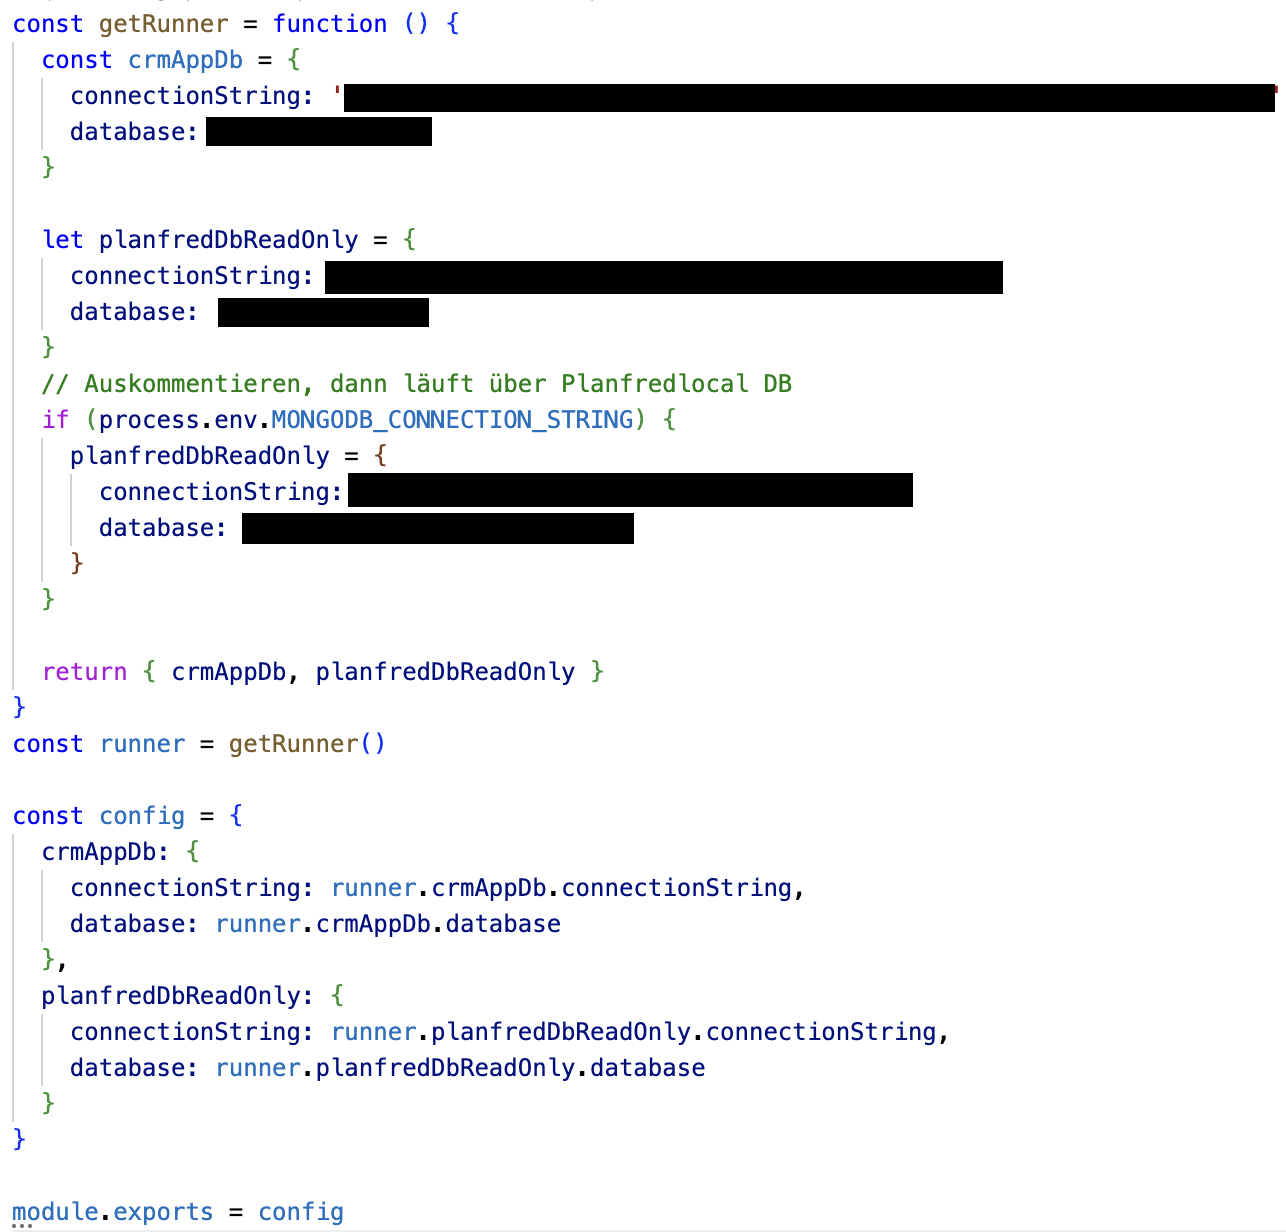
\includegraphics[width=0.5\textwidth]{pics/config-file-conn-strings.png}
    \caption{Config-File}
    \label{fig:enter-label}
\end{figure}
\newline
Wie man im obigen Screenshot erkennen kann, ist noch die Möglichkeit implementiert, durch Auskommentieren des if-Statements, auf eine Datenbank zuzugreifen, welche weniger Einträge enthält.
\newline
Anschließend wird in einem weiteren File dieses JSON importiert und eine Funktion erstellt, in welcher, wie im oben gezeigten Beispiel, die Verbindung aufgebaut wird.
\begin{lstlisting}
async connect () {
    const client = new MongoClient(this.dbConfig.connectionString)
    const result = await client.connect()
    this.db = result.db(this.dbConfig.database)
    logger.info(`Connected to MongoDB ${this.dbConfig.database}.`)
}
\end{lstlisting}
Diese Funktion wird ebenfalls exportiert und im server.js importiert und aufgerufen. Dabei wird jeweils auf den erfolgreichen Verbindungsaufbau gewartet, damit es nicht zu dem Fehler kommen kann, dass eine der Datenbanken nicht verbunden ist. Sind beide Datenbanken erfolgreich verbunden, wird der Server gestartet.